%%%%%%%%%%%%%%%%%%%%%%%%%%%%%%%%%%%%%%%%%
% Beamer Presentation
% LaTeX Template
% Version 1.0 (01/07/19)
%
%%%%%%%%%%%%%%%%%%%%%%%%%%%%%%%%%%%%%%%%%

%----------------------------------------------------------------
%	PACKAGES AND THEMES		-----------------------------------
%----------------------------------------------------------------

\documentclass[xcolor=table,11pt]{beamer}

\mode<presentation> {
	
	\usetheme{Frankfurt}
	\usecolortheme{dove}
	\usefonttheme{serif}
	
}
\usepackage{newtxtext,newtxmath}
\usepackage{graphicx}
\usepackage{booktabs} 
\usepackage{subfig}
\usepackage{pgf}
\usepackage{multirow}
\usepackage{appendixnumberbeamer}
\usepackage{bookmark}
\usepackage{siunitx}
\usepackage{animate}
\usepackage{xcolor}
\usepackage{soul}
\usepackage{pifont}
\usepackage{caption}
\usepackage{array}
\usepackage{pgffor}
\usepackage{tabularx}
\captionsetup{skip=0pt,belowskip=0pt}


%----------------------------------------------------------------
%	GENERAL OPTIONS 	-----------------------------------------
%----------------------------------------------------------------

% Set template options
\setbeamertemplate{section in toc}{\inserttocsectionnumber.~\inserttocsection}
\setbeamertemplate{frametitle}{\vspace*{1em}\insertframetitle}
\setbeamertemplate{enumerate items}[default]
\setbeamercolor{section in head/foot}{fg=white, bg=black}
\setbeamercolor{normal text}{fg=white,bg=black}

% Headline
\makeatletter
\setbeamertemplate{headline}
{%
	\pgfuseshading{beamer@barshade}%
	\vskip-5ex%
	\begin{beamercolorbox}[ignorebg,ht=2.25ex,dp=3.75ex]{section in head/foot}
		\insertsectionnavigationhorizontal{\paperwidth}{\hskip0pt plus1fill}{\hskip0pt plus1fill}
	\end{beamercolorbox}%
	\ifbeamer@sb@subsection%
	\begin{beamercolorbox}[ignorebg,ht=2.125ex,dp=1.125ex,%
		leftskip=.3cm,rightskip=.3cm plus1fil]{subsection in head/foot}
		\usebeamerfont{subsection in head/foot}\insertsubsectionhead
	\end{beamercolorbox}%
	\fi%
}%
\makeatother

% Footline
\makeatletter
\setbeamertemplate{footline}
{
	\leavevmode%
	\hbox{%
		\begin{beamercolorbox}[wd=.333333\paperwidth,ht=2.25ex,dp=1ex,left]{section in head/foot}%
			\usebeamerfont{author in head/foot}\hspace{10pt}\insertshortauthor
		\end{beamercolorbox}%
		\begin{beamercolorbox}[wd=.333333\paperwidth,ht=2.25ex,dp=1ex,center]{section in head/foot}%
			\usebeamerfont{title in head/foot}\insertshorttitle
		\end{beamercolorbox}%
		\begin{beamercolorbox}[wd=.333333\paperwidth,ht=2.25ex,dp=1ex,right]{section in head/foot}%
			\usebeamerfont{date in head/foot}\insertshortdate{}\hspace*{2em}
			\insertframenumber{}\hspace*{2em}
	\end{beamercolorbox}}%
	\vskip0pt%
}
\makeatother

% Add logo
\logo{\pgfputat{\pgfxy(0,7)}{\pgfbox[right,base]{
\includegraphics[width=0.1\paperwidth]{Unibe_Logo}}}}
% \titlegraphic{\includegraphics[width=0.5\paperwidth]{Pictures/ESB_2023}}

% Table settings
\renewcommand{\arraystretch}{2}
\captionsetup{labelformat=empty,labelsep=none}
\definecolor{Gray}{gray}{0.9}

% Define highlitghing command
\makeatletter
\let\HL\hl
\renewcommand\hl{%
	\let\set@color\beamerorig@set@color
	\let\reset@color\beamerorig@reset@color
	\HL}
\makeatother

% Add overview at each begin of section
%\AtBeginSection[]
%{
	%	\begin{frame}
		%		\frametitle{Overview}
		%		\tableofcontents[currentsection]
		%	\end{frame}
	%}


\renewcommand{\arraystretch}{1.4}
\newcommand{\ColWidth}{1}
\newcommand{\TrimSize}{50}

%----------------------------------------------------------------
%	TITLE PAGE 	-------------------------------------------------
%----------------------------------------------------------------

\title[FABCORT]{Fabric-Elasticity Relationships in Cortical Bone} 

\author[mathieu.simon@unibe.ch]{\tiny{\bf{Mathieu Simon}}}

\medskip
\date{December, 2024}

\begin{document}
	
	\begin{frame}
		\titlepage
	\end{frame}
	
	%----------------------------------------------------------------
	%----------------------------------------------------------------
	%----------------------------------------------------------------
	
	\section{Material and Methods}

	\begin{frame}
		\frametitle{Material}
		\begin{columns}
			\column{0.4\linewidth}
			\vfill

			Data
			\begin{itemize}
				\item 59 scans
				\item 6.5 \textmu m voxel size
				\item RUS measurements
				\item CTAnalyser
			\end{itemize}
			\vfill

			\column{0.3\linewidth}
			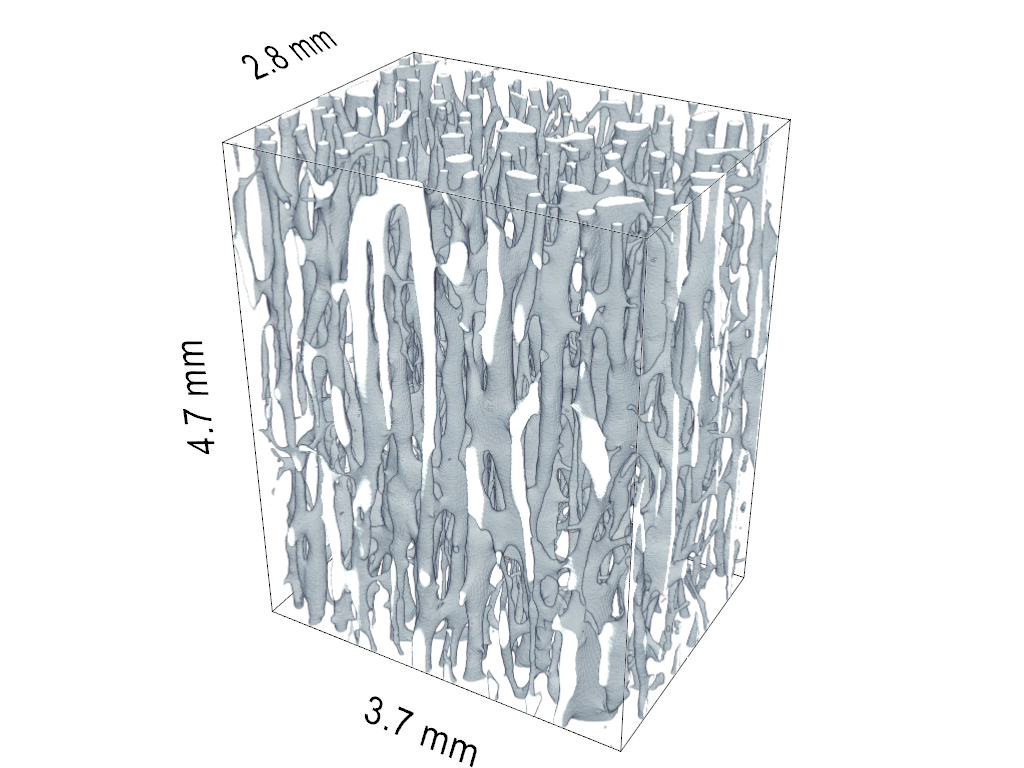
\includegraphics[width=\linewidth, trim=200 0 0 0]{01_Fabric/Plots/Scan}\\
			
			\column{0.3\linewidth}
			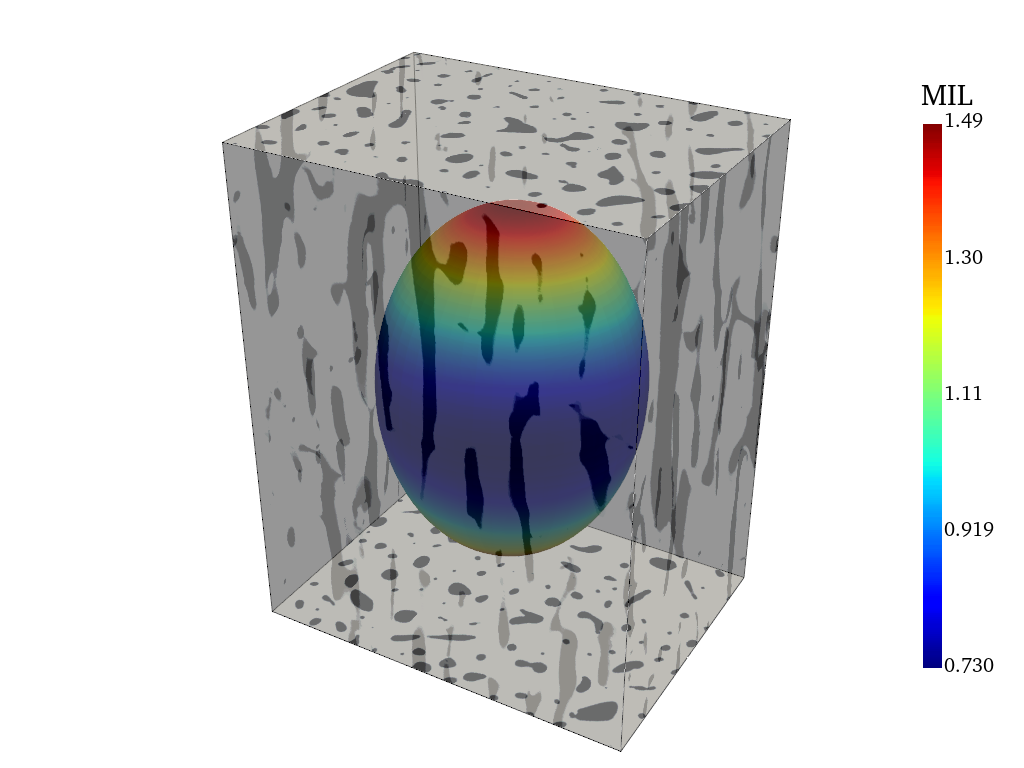
\includegraphics[width=\linewidth, trim=200 0 0 0]{01_Fabric/Plots/Fabric}\\

		\end{columns}
	\end{frame}

	\begin{frame}
		\frametitle{Segmentation}

		\begin{columns}

			\column{0.3\linewidth}
			\vfill
			\centering
			Mean Otsu threshold\\
			\vfill
			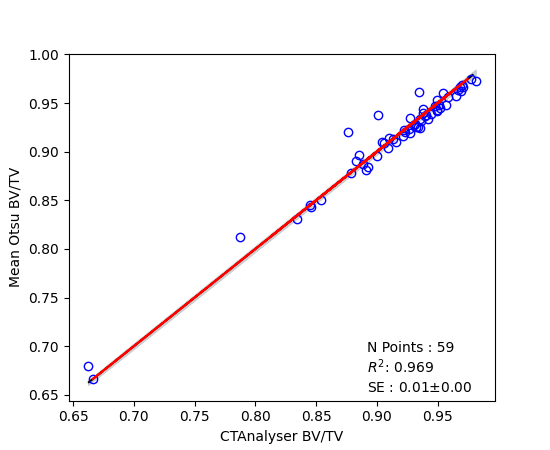
\includegraphics[height=3.75cm, trim=50 0 0 0]{01_Fabric/Results/BVTV_OLS}\\
			\vfill

			\column{0.5\linewidth}
			\vfill
			\centering
			Fabric distribution\\
			\vfill
			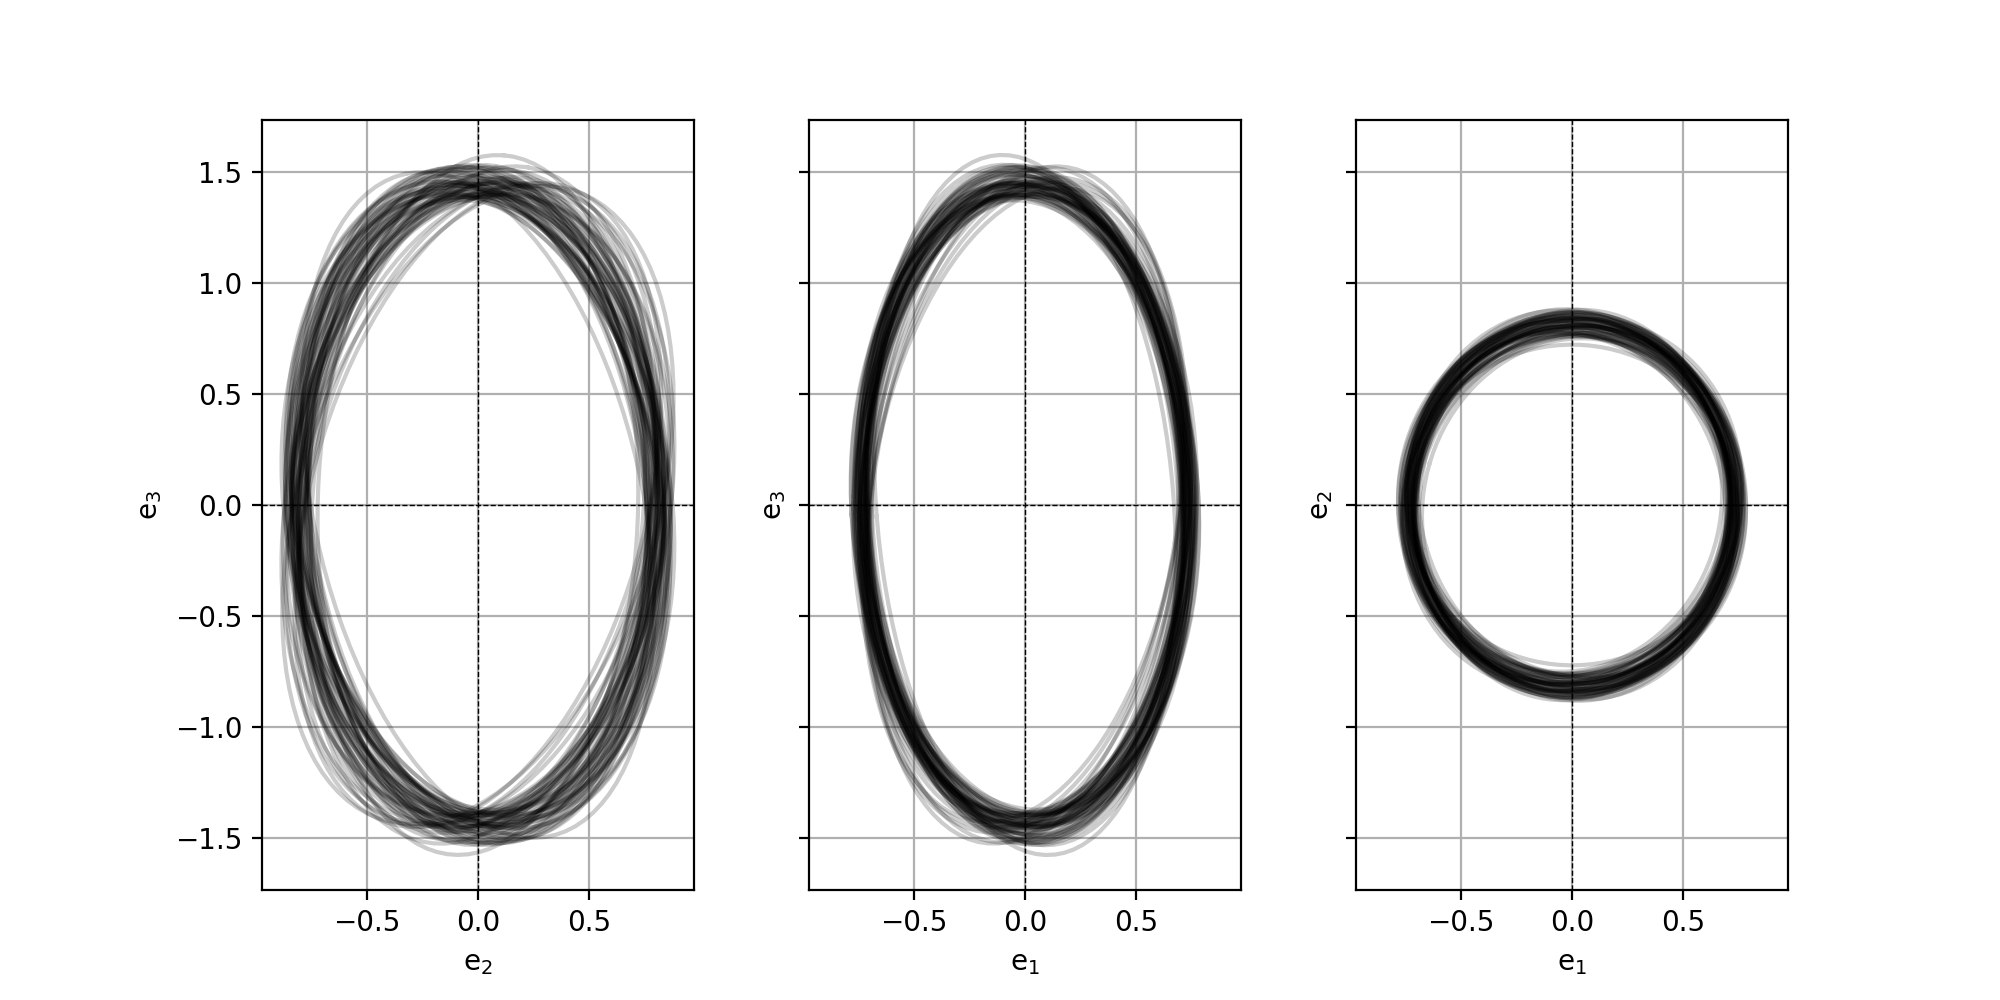
\includegraphics[height=3.75cm, trim=100 0 0 0]{01_Fabric/Results/Fabric}\\
			\vfill
			
		\end{columns}
	
	\end{frame}

	\begin{frame}
		\frametitle{Resolution Effect - Fabric}

		\begin{columns}
			\column{0.5\linewidth}
			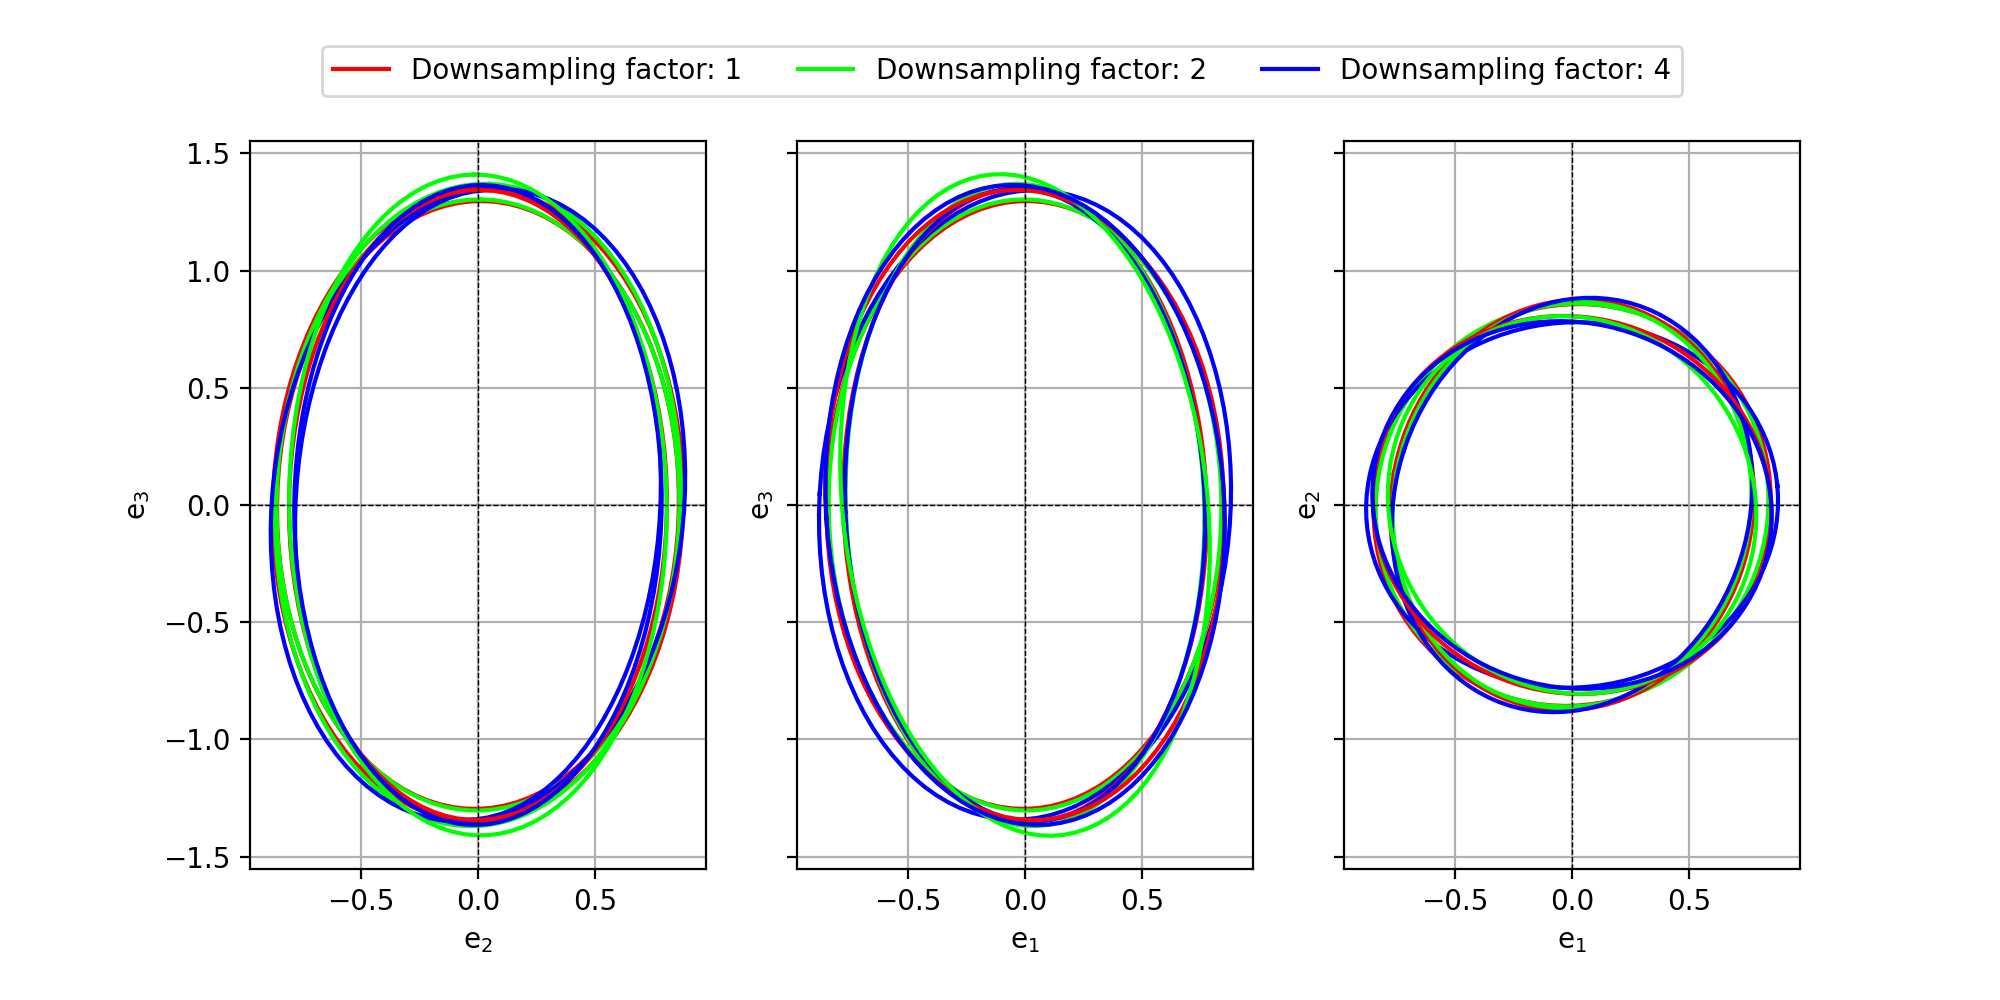
\includegraphics[height=3.25cm]{02_ResolutionEffect/Results/Fabric}\\

			\column{0.5\linewidth}
			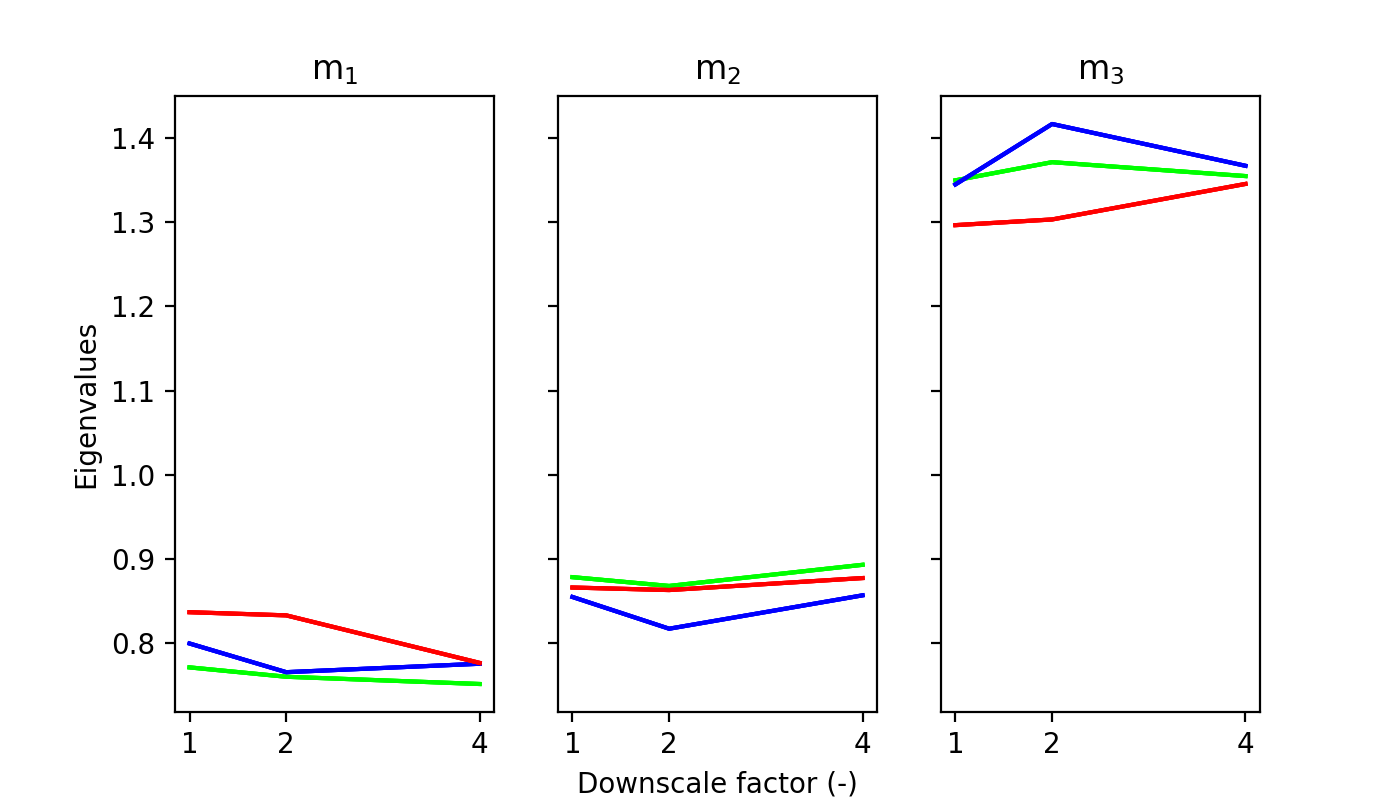
\includegraphics[height=3.25cm]{02_ResolutionEffect/Results/eValues}\\
		\end{columns}

	\end{frame}

	\begin{frame}
		\frametitle{Resolution Effect - Elasticity}
		\centering
		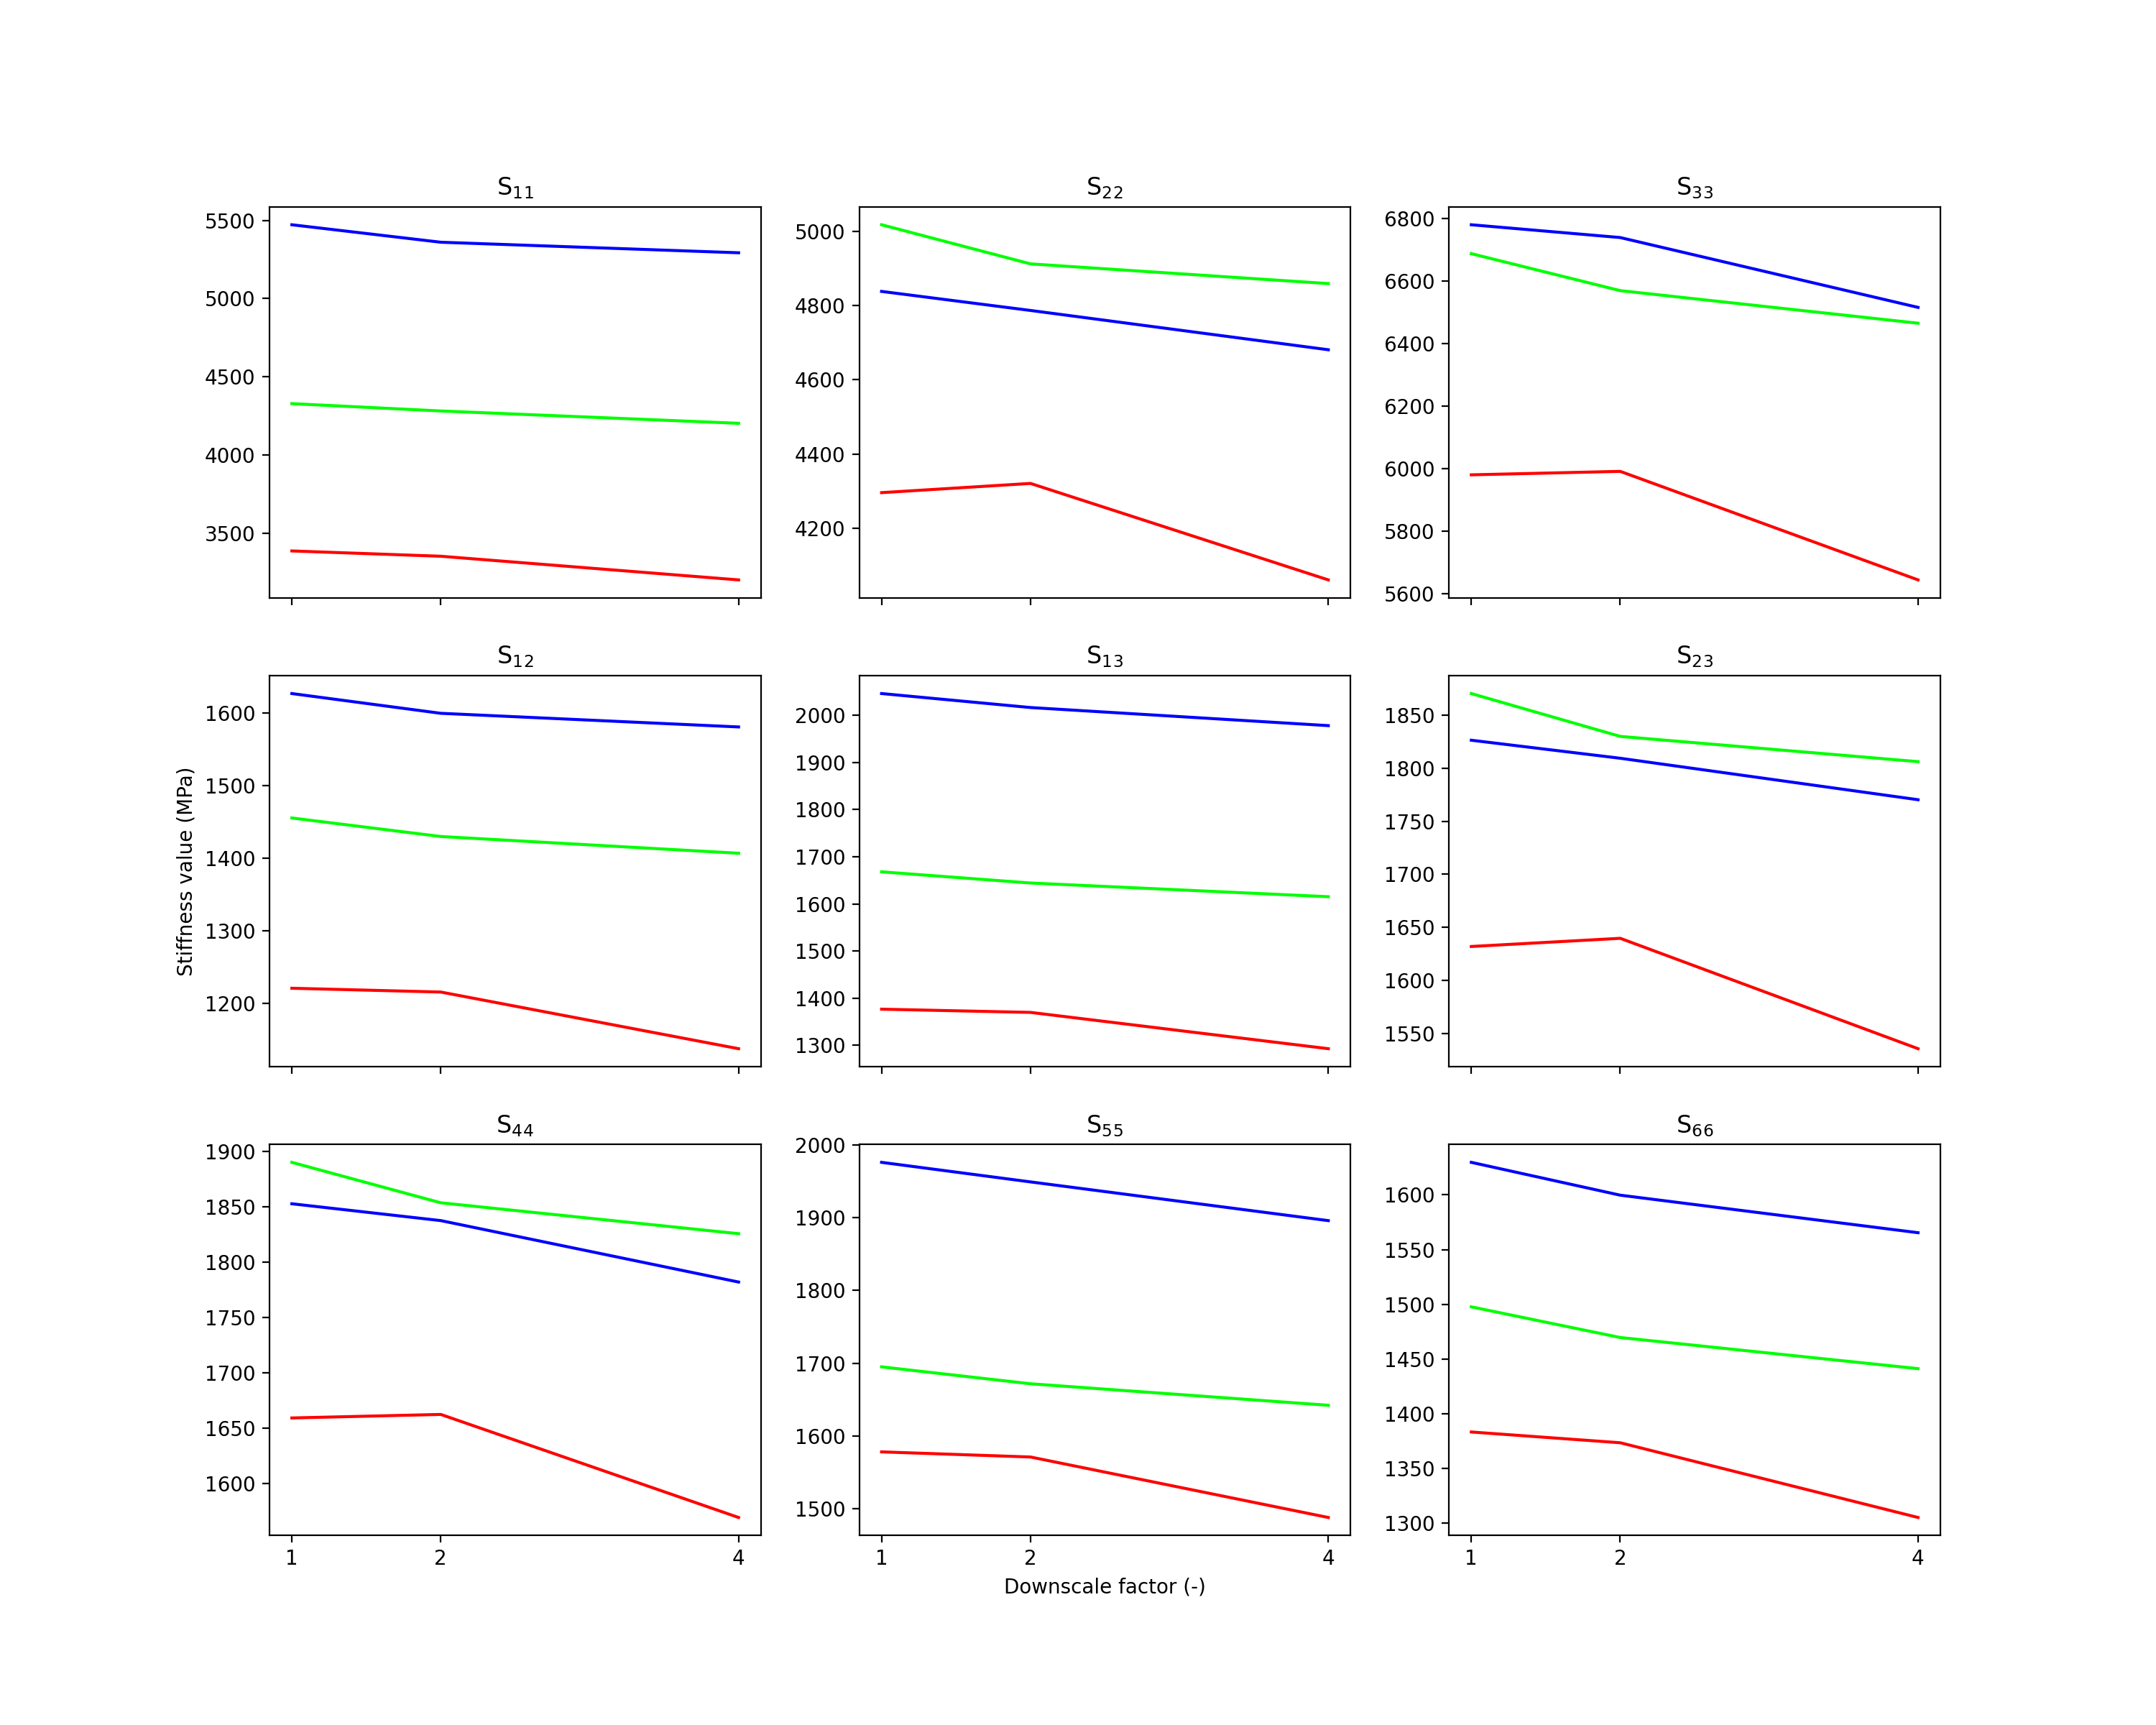
\includegraphics[height=7.5cm, trim=0 0 0 20]{02_ResolutionEffect/Results/Stiffness}\\
	\end{frame}

	\begin{frame}
		\frametitle{Resolution Effect - Elasticity II}

		\begin{columns}
			\column{0.5\linewidth}
			\centering
			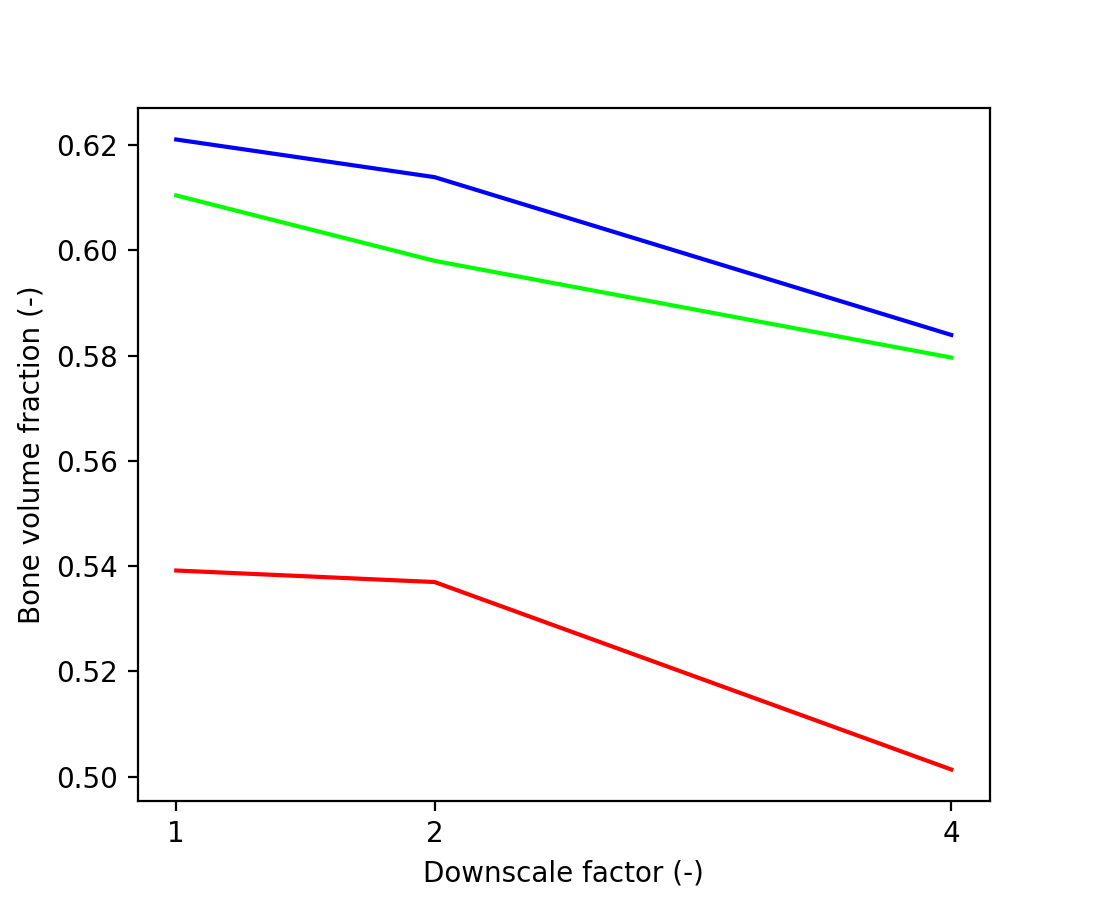
\includegraphics[height=5cm]{02_ResolutionEffect/Results/BVTV_Downscaling}\\

			\column{0.5\linewidth}
			\centering
			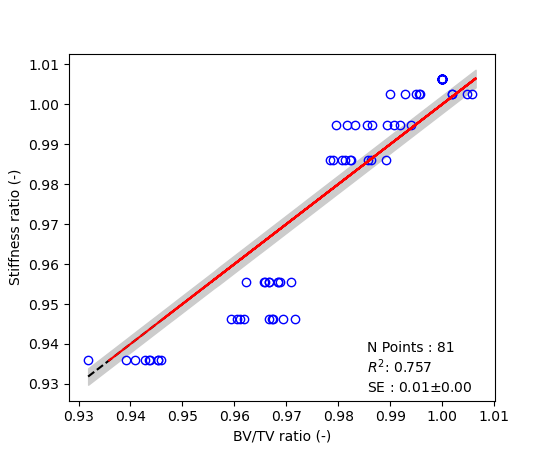
\includegraphics[height=5cm]{02_ResolutionEffect/Results/BVTV_Stiffness}\\
		\end{columns}

	\end{frame}

	\begin{frame}
		\frametitle{Convergence Study}

		\begin{columns}
			\column{0.5\linewidth}
			\vfill

			Setup
			\begin{itemize}
				\item 1mm ROI side length
				\item 3x3x5 ROIs
				\item 65 \textmu m margin
				\item Groups of 1, 2, ..., 45 ROIs
			\end{itemize}
			$\rightarrow$ \textasciitilde 2\textsuperscript{45} possibilities
			\vfill

			\column{0.4\linewidth}
			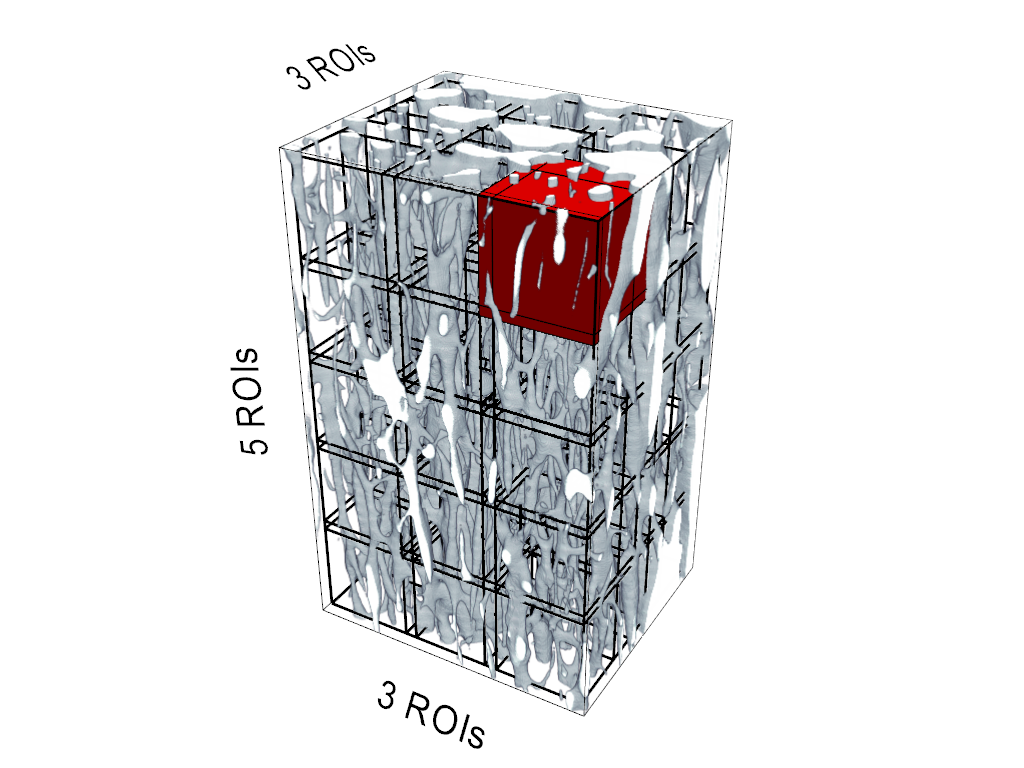
\includegraphics[width=\linewidth, trim=200 0 0 0]{03_ConvergenceStudy/Results/ROIs}\\

		\end{columns}

	\end{frame}

	\begin{frame}
		\frametitle{Convergence Study}

		\begin{columns}
			\column{0.5\linewidth}
			\vfill

			Sampling
			\begin{itemize}
				\item Balanced clustering\\
					  $\rightarrow$ Linear sum assignment\\
					  $\rightarrow$ 216*10\textsuperscript{6} possibilities
				\item N samples = 1000
				\item Norm Error
				\item Threshold = 0.05
			\end{itemize}
			$\rightarrow$ 15-16 ROIs
			\vfill

			\column{0.4\linewidth}
			\vfill
			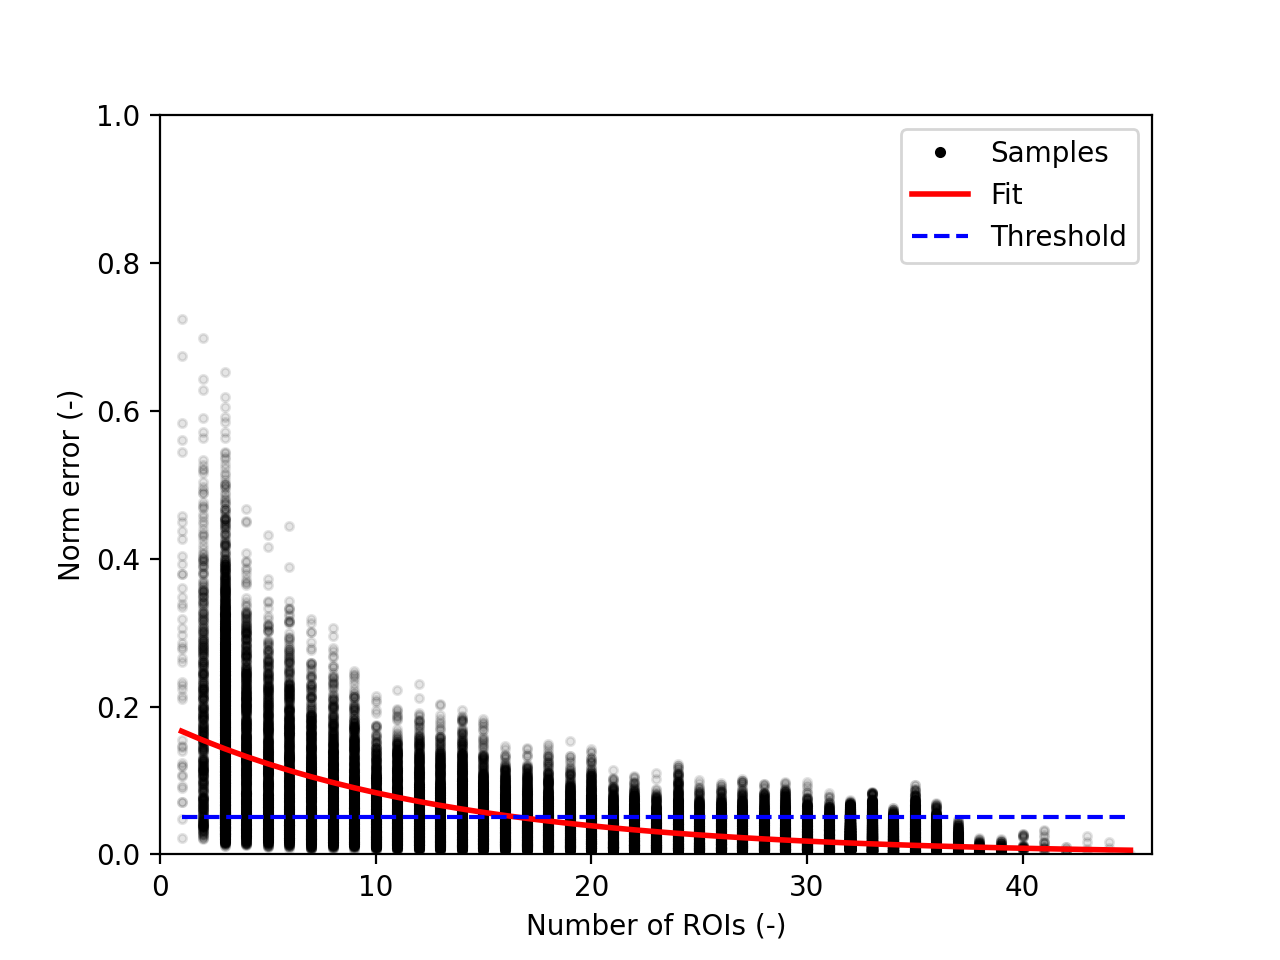
\includegraphics[width=\linewidth, trim=75 0 0 0]{03_ConvergenceStudy/Results/NormError}\\
			\vfill

		\end{columns}

	\end{frame}

	\begin{frame}
		\frametitle{Material Effect}
		\vfill
		\includegraphics[width=\linewidth]{04_MaterialEffect/Material}\\
		\vfill
	\end{frame}

	\begin{frame}
		\frametitle{Homogenization}

		\begin{columns}
			\column{0.5\linewidth}
			\vfill
			Setup
			\begin{itemize}
				\item Downsampling factor: 2
				\item 16x1mm\textsuperscript{3} ROIs
				\item Isotropic vs transverse
				\item Mean $\mathbb{S}$ / Sample
			\end{itemize}
			\vfill

			\column{0.4\linewidth}
			\vfill
			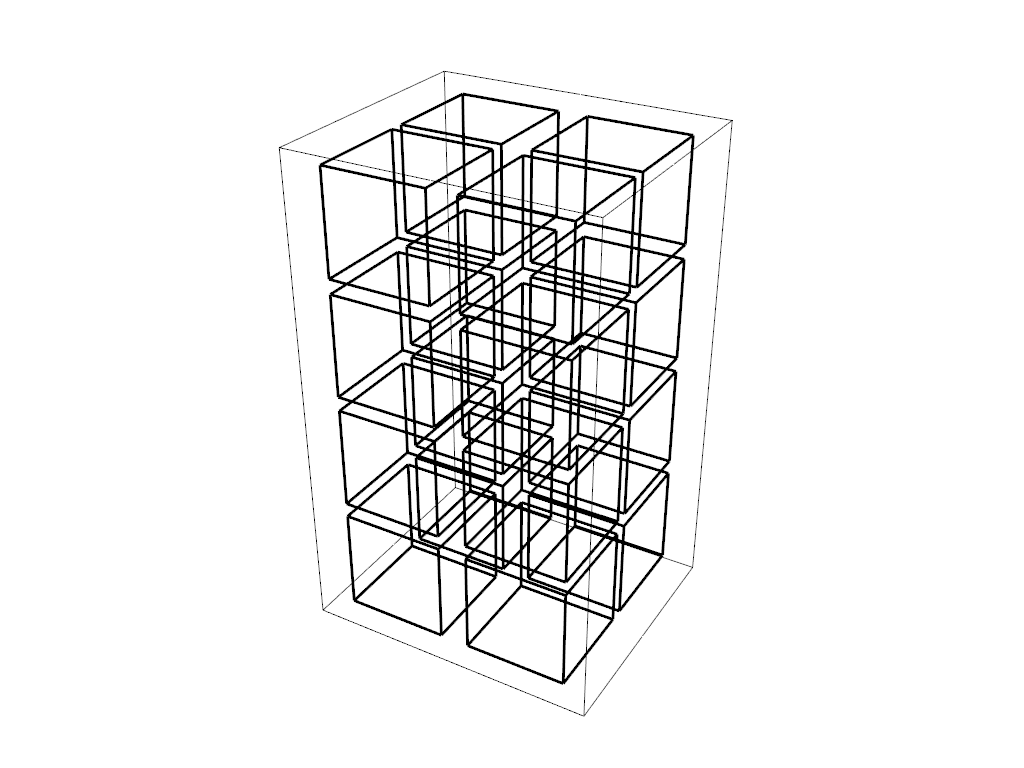
\includegraphics[width=\linewidth, trim=200 0 0 0]{05_Homogenization/Plots/ROIs}\\
			\vfill

		\end{columns}
	\end{frame}

	\begin{frame}
		\frametitle{Homogenization - Comparison with RUS}
		\vfill
		\hfill 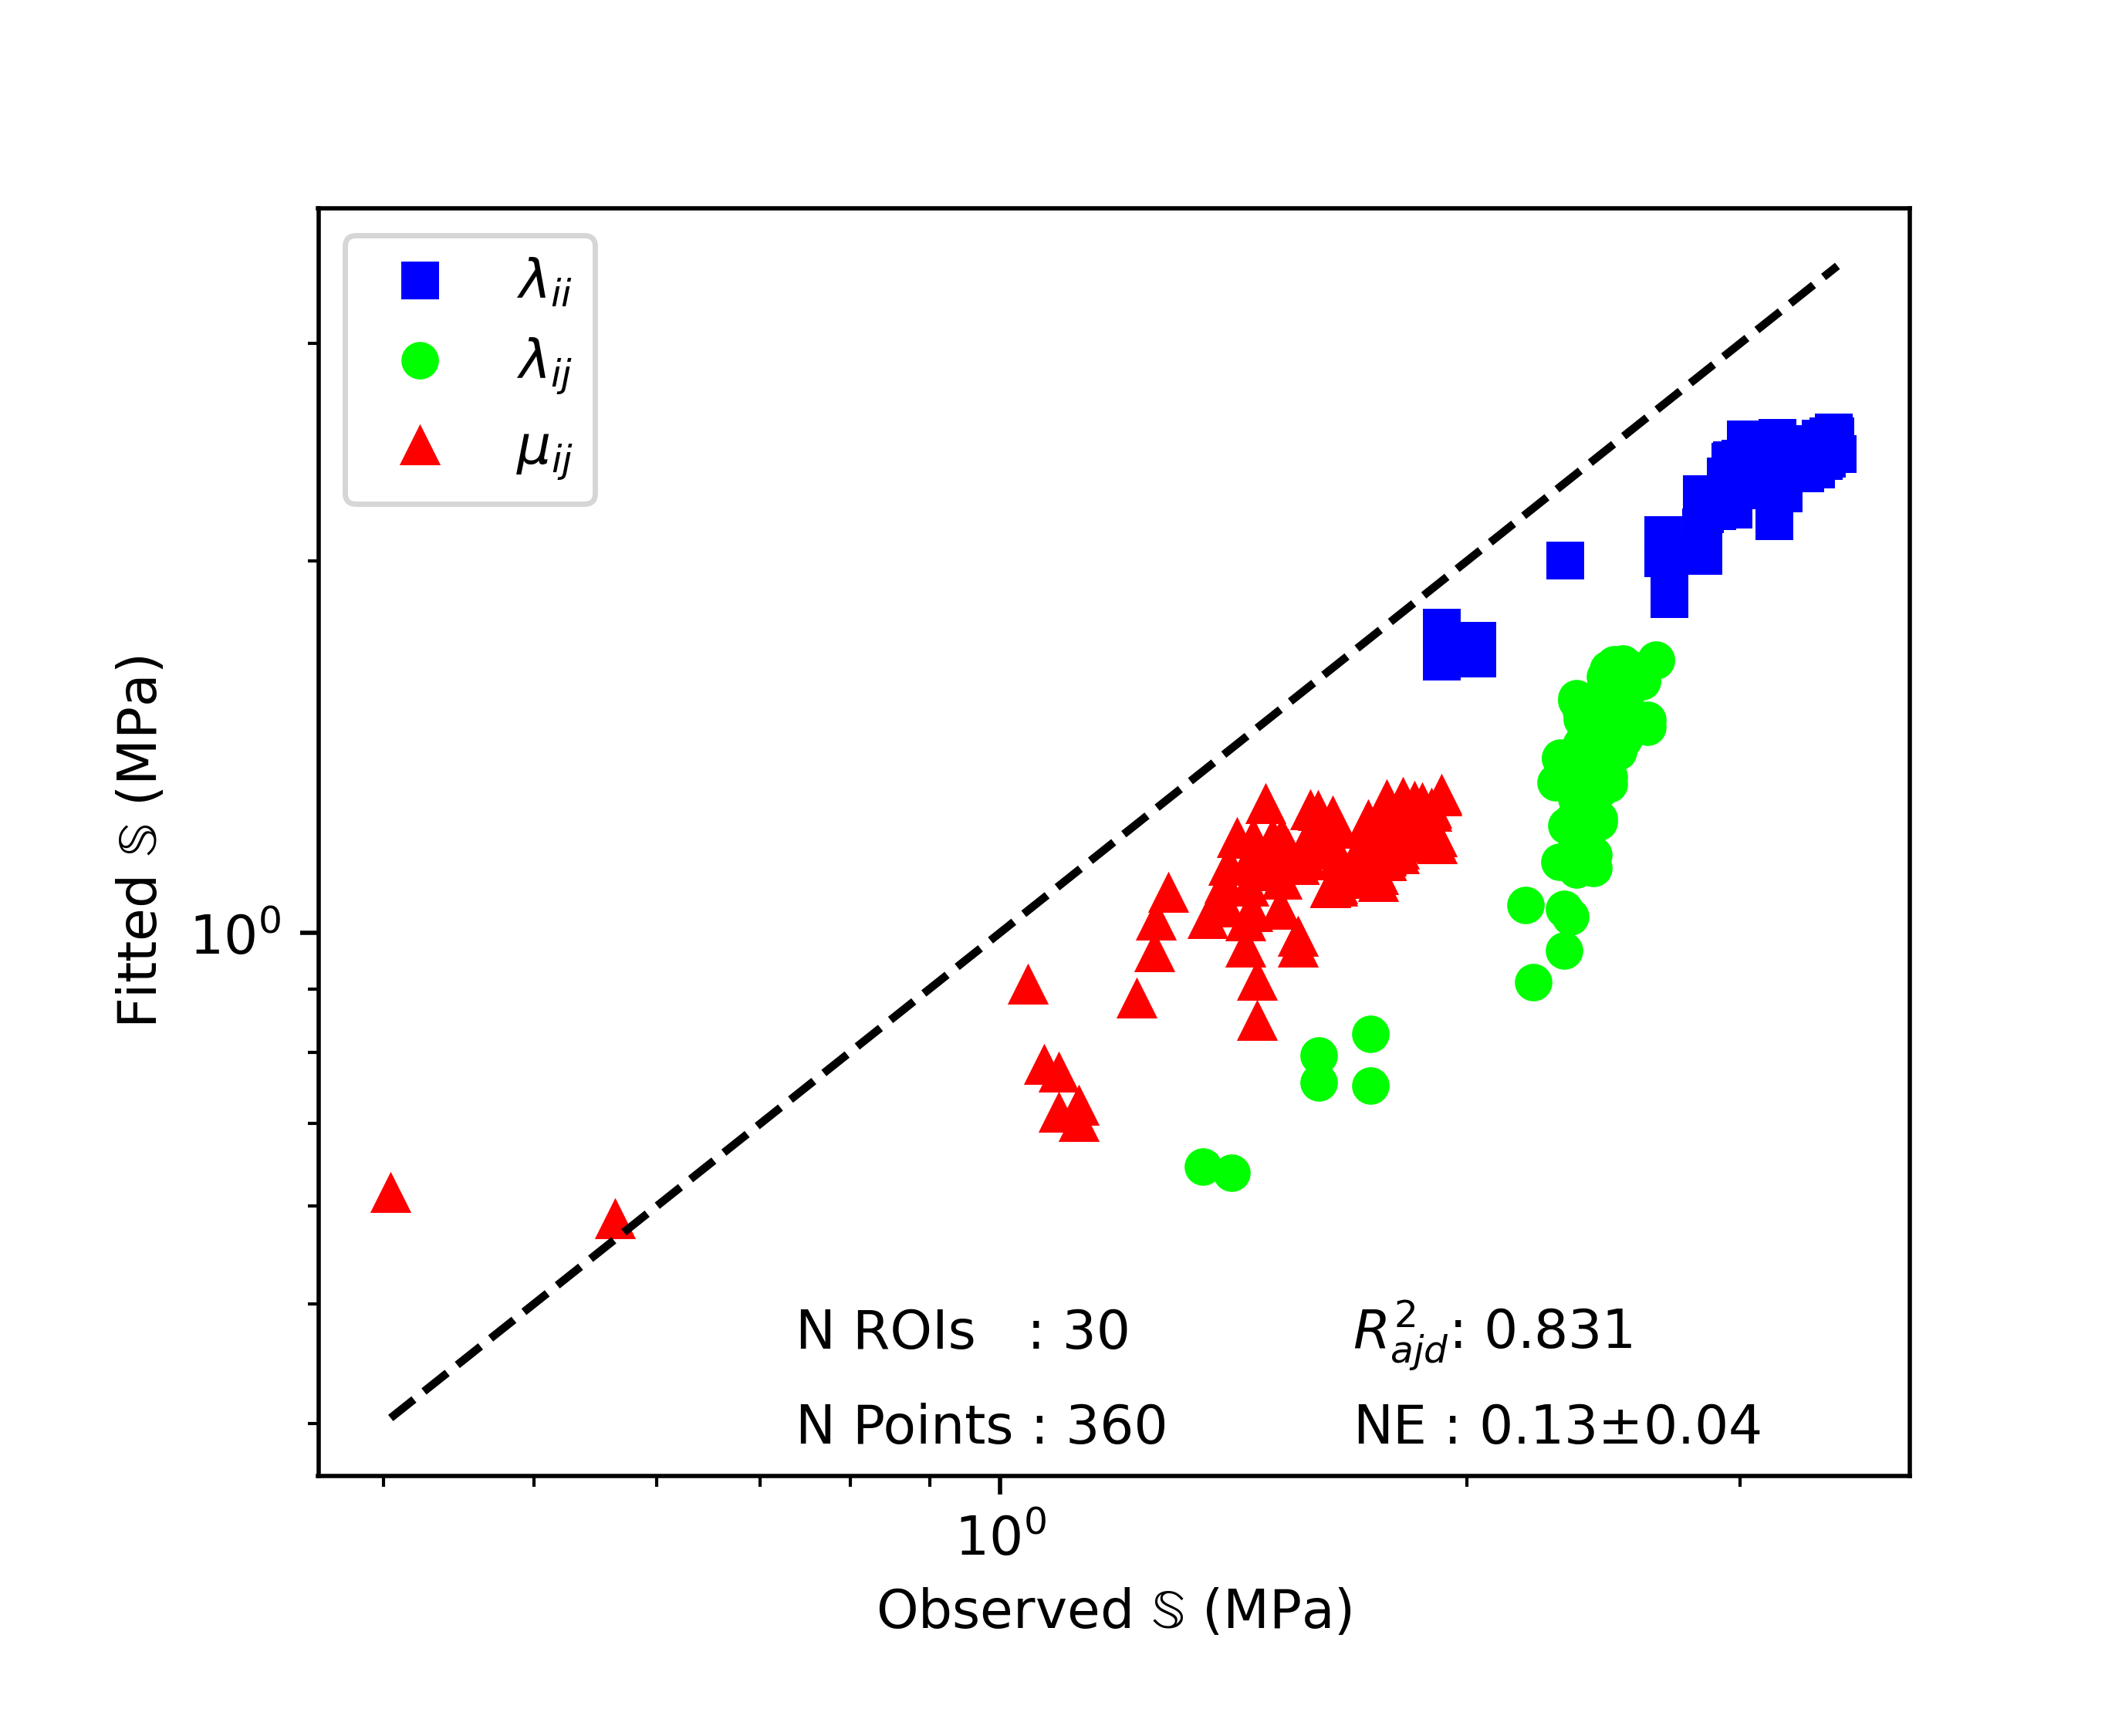
\includegraphics[width=0.4\linewidth]{05_Homogenization/Plots/Elasticity_IsoRUS}
		\hfill 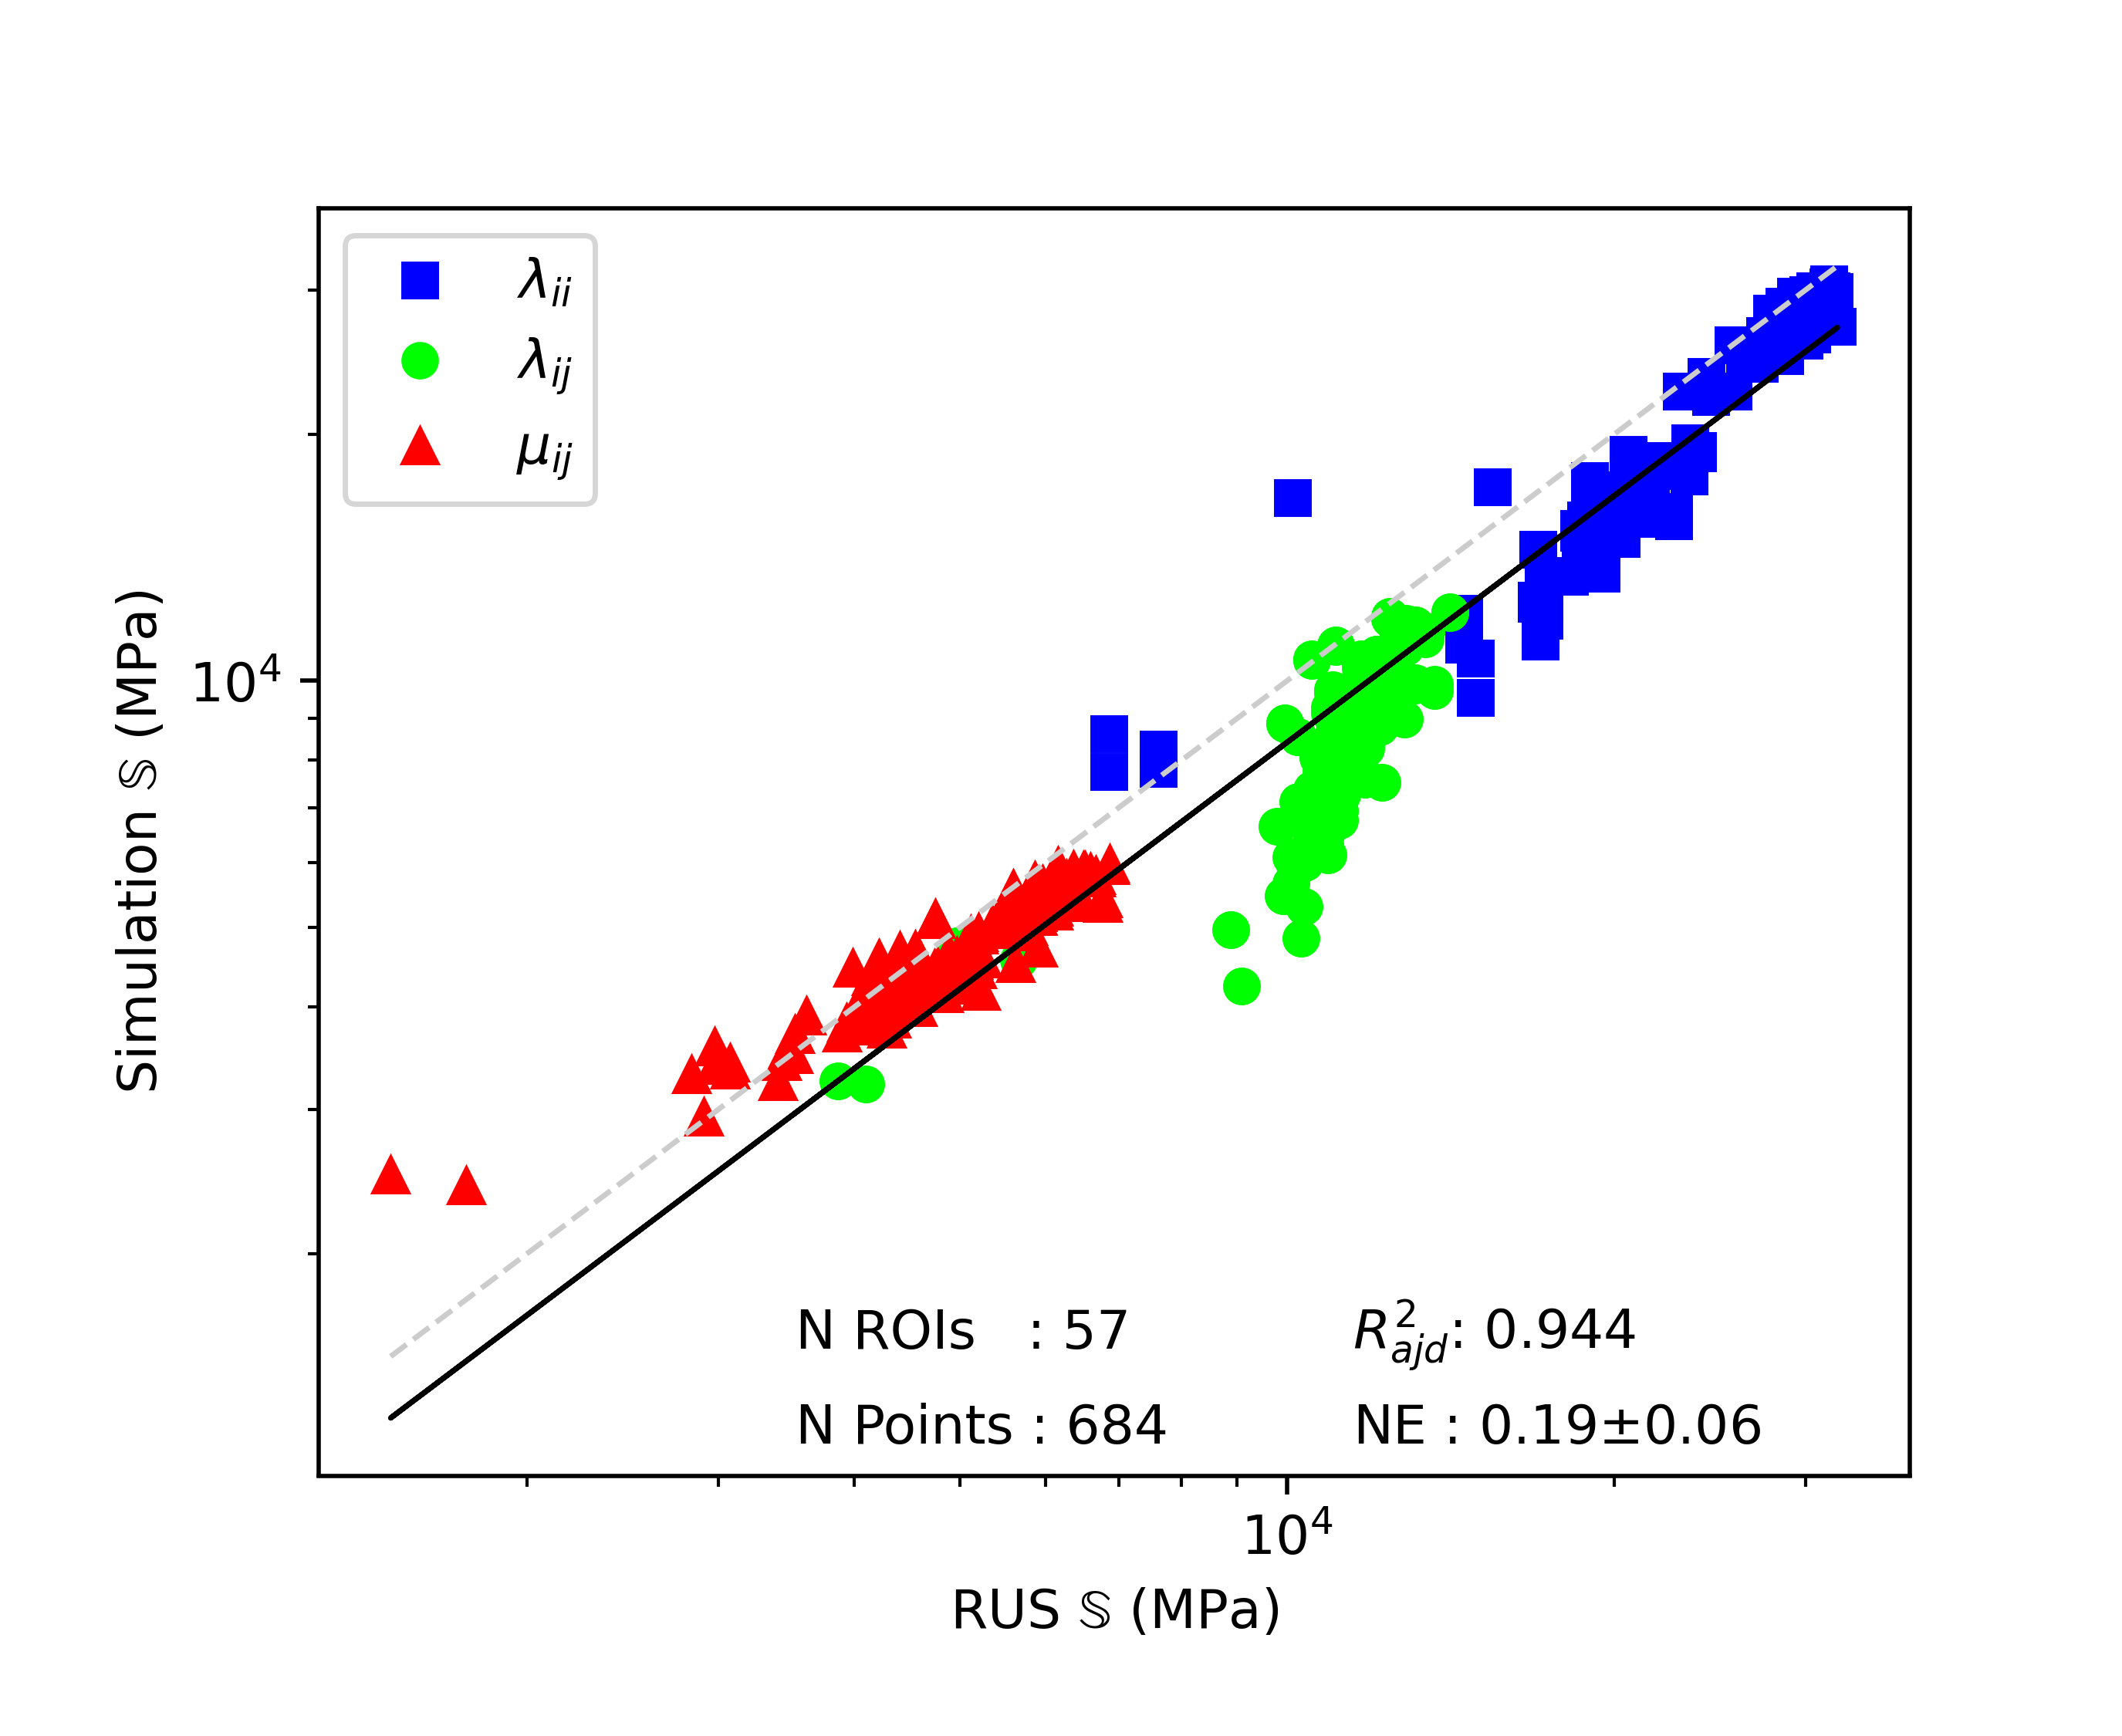
\includegraphics[width=0.4\linewidth]{05_Homogenization/Plots/Elasticity_TraRUS}
		\hfill\\
		\hfill Isotropic Material \hfill Transverse Isotropic Material \hfill\\
		\vfill
	\end{frame}
		
	\begin{frame}
		\frametitle{Homogenization - Isotropic}

		\begin{columns}
			\column{0.5\linewidth}
			Setup
			\begin{itemize}
				\item Fabric at original resolution
				\item BV/TV at original resolution
				\item Isotropic material
				\item Mean $\mathbb{S}$ / Sample
			\end{itemize}
			\vspace{5mm}
			Parameters:
			\resizebox{\linewidth}{!}{%
			\begin{tabular}{ccccc}
				$\lambda_0$ & $\lambda_0'$ & $\mu_0$ & $k$ & $l$\\
				3132 & 4944 & 4944 & 1.978 & 0.121 \\
			\end{tabular}}

			\column{0.4\linewidth}
			\vfill
			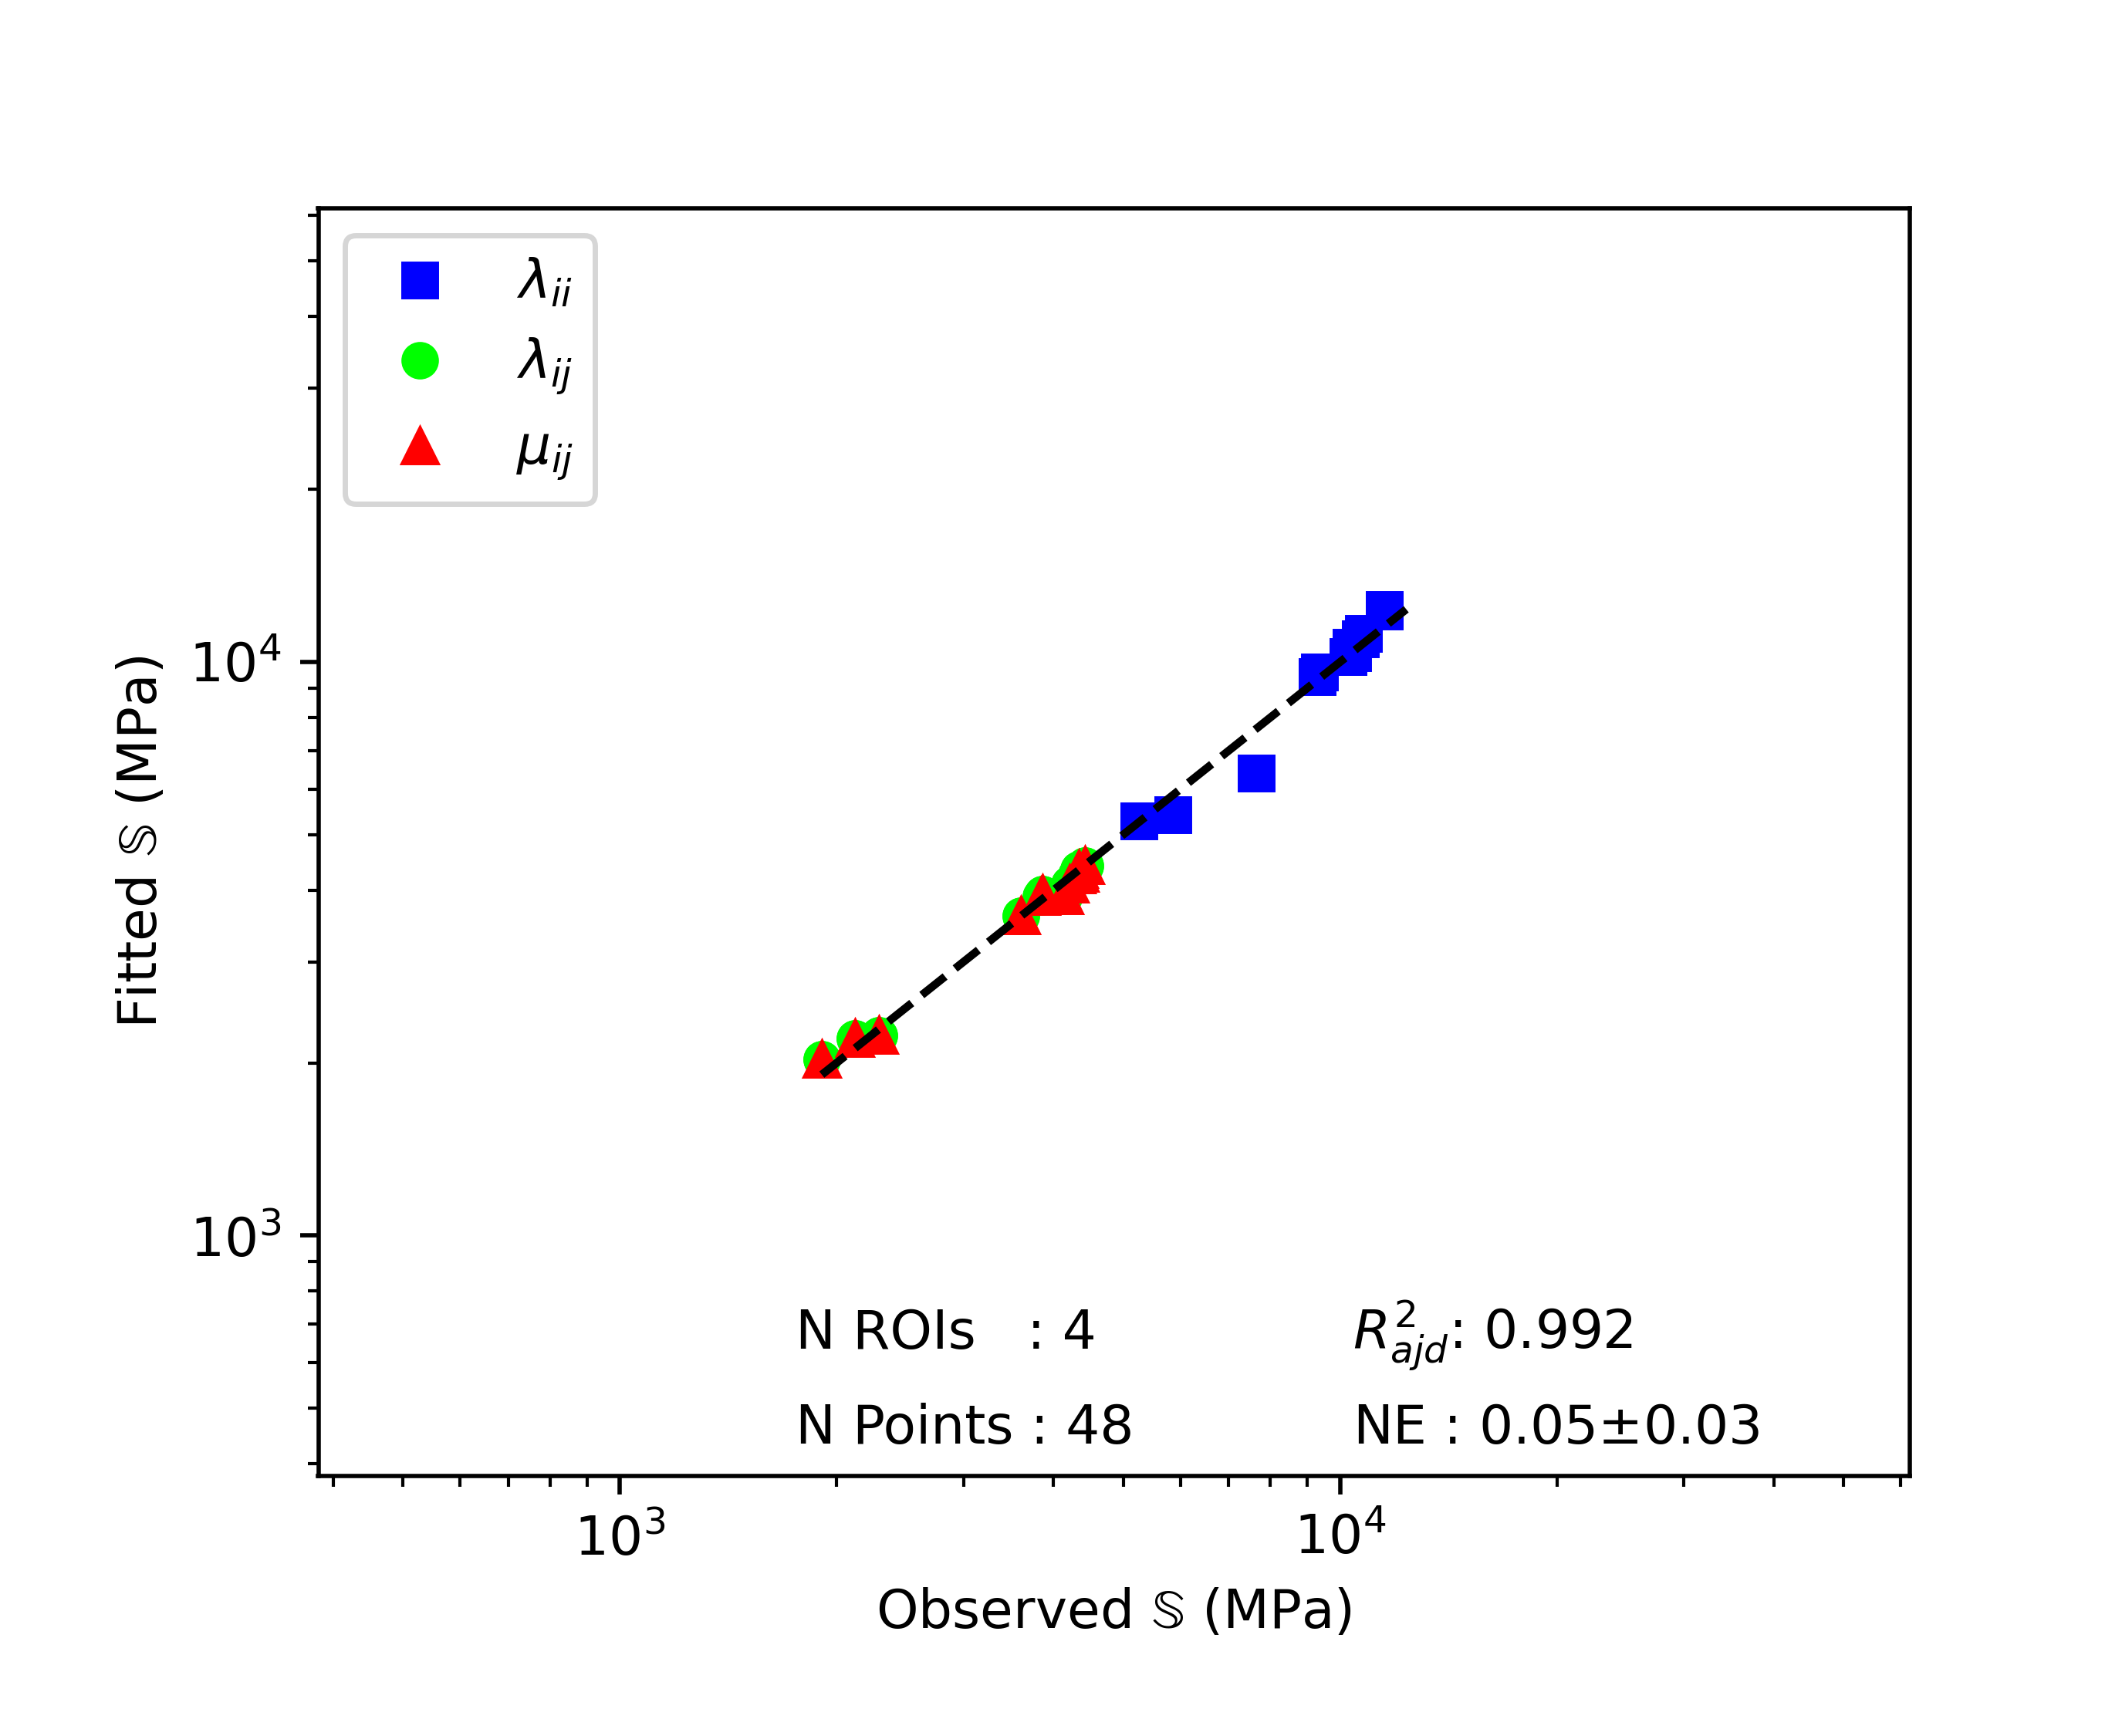
\includegraphics[width=\linewidth, trim=75 0 0 0]{05_Homogenization/Plots/FabricElasticity_Iso}\\
			\vfill

		\end{columns}
	\end{frame}
	%----------------------------------------------------------------
	%----------------------------------------------------------------
	%----------------------------------------------------------------

\end{document}